\todopar{Discuss the Mephisto laser head. Laser basics. Non-planar
ring oscillator. Beam shape. Frequency and intensity noise.
}
\section{Intensity Stabilization}
\todopar{Paragraph on the theory of operation}
\subsection{Sensing}
\todopar{Photo-electric effect, quantum efficiency}

\subsection{Feedback}
\todopar{Electronics}

\subsection{Actuation}
\todo{Description of Acousto-Optic Modulator}


\section{Frequency Stabilization}

\subsection{Sensing}
\subsubsection{Cavity Assembly}
\subsubsection{Cavity Suspension}
\begin{figure}[htbp]
	\centering
		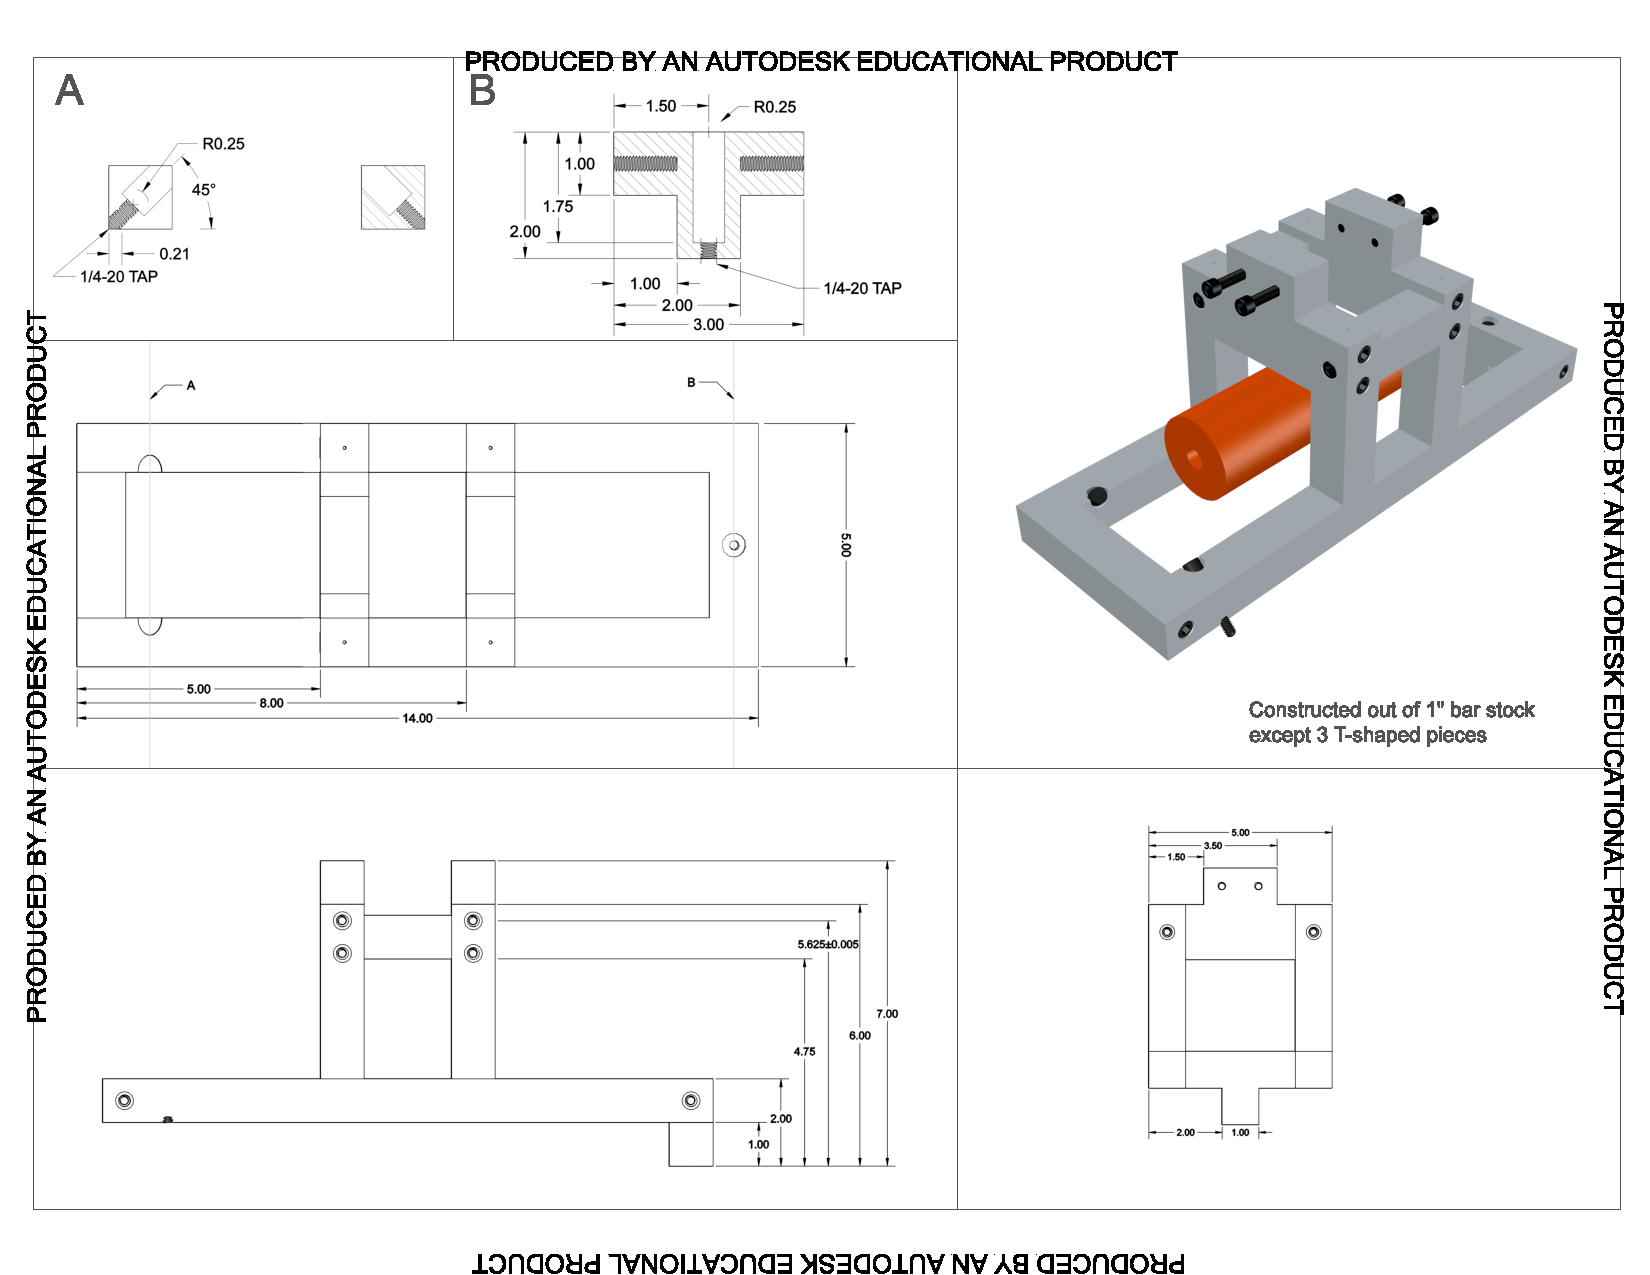
\includegraphics[width=15cm]{./figures/refcavsusdesign.pdf}
	\caption[Reference Cavity Suspension Design]{Design of the reference cavity suspension}
	\label{fig:refcav_sus}
\end{figure}

\subsubsection{PDH Locking}

\subsection{Feedback}

\subsection{Actuation}

\todopar{Add a description of the Electro-Optic Modulator}

\subsubsection{Laser Head Thermal}

\subsubsection{Laser Head Piezo-Electric Transducer}
\todopar{add description of peizo-electric effect}
\todopar{describe the effects of the piezo in-loop}

\section{Mode Cleaner}
\todopar{add description of PMC, reference Willke,98}

\subsection{Sensing}

\subsection{Feedback}

\subsection{Actuation}
